%!Tex root = main.tex
In order to understand how humans evaluate MT, we ran an evaluation experiment using \eye, involving $20$ human participants, half of them \mono in English and the other half \bil in Spanish-English. We chose the Spanish-English language pair because of the large amount of freely available data (e.g. WMT) and the sizable pool of available participants in our environment. In our setup, we contrasted the evaluation procedure under alternative \gamets in which different sources of information (e.g. source sentence, reference translation) are available.  To keep things simple, we only asked participants to evaluate one translation at a time and provide a single score representing the translation quality. To prevent biasing the behavior of the participants, and to encourage them to evaluate translations \emph{naturally}, participants were not given any precise instructions regarding the requirements of a \emph{good} translation. To increase engagement, we formulated the evaluation experiment as a game, where participants are provided feedback after each evaluation according to how close their own score was to a precomputed quality score. Below, we further describe the data used, the different \gamets, the background of the participants, and other details of our experiment. %participants read different combinations of translation evaluation data using the open-source MT evaluation platform Appraise ~\cite{federmann2012appraise} and give an evaluation score, while an eye-tracking device ~\cite{eyetribe2014settingup} is recording their eye movements. As variables, we analyse the time participants spend in specific areas of interest, and the scores they give to translations. 

\subsection{Data}
%!TEX root = main.tex
In our experiments we used the WMT12 \cite{WMT12} human evaluation data for Spanish-English systems. The data consists of $1141$ ranking annotations, in which each evaluator ranked %$5$ 
five out of the $12$ participating systems. \\
The annotation effort generated a total of $5705$ labels with an inter-annotator agreement of $\kappa=0.222$. Unfortunately, many of the translations have rankings coming from a single evaluator only. %, which means that from many sentences only 5 out of 12 systems were ranked. Therefore, to have more reliable data, we only included sentences for which there were at least $1.25$ labels per system. %More specifically, we discarded sentences with an average number of labels per system below $1.25$. 
In practical terms, this means that at least two evaluators had to evaluate the translations of the same source sentence, and 
%for a given source sentence with ranking evaluations by two different users, we required that 
at least two systems were ranked by both of those evaluators.
In the WMT12 data, a total of $923$ different source sentences were evaluated. % yet only $177$ had evaluations from more than $1$ judge. 
From these, we kept only the $155$ that complied with our requirement. 

\vspace{5pt}
To control for length (i.e number of words), we divided the sentences into three equally sized groups based on the sentence length of their reference translations.  Discarding the five longest ones the resulting sets \llong, \lmid, and \lshort averaged $30.88$, $18.18$, and $10.18$ words.
\vspace{5pt}

To have diversity in the quality of the translations, 
%we included translations of different levels of translation quality according to the human rankings. Therefore, 
we collected two translations per source sentence, one of superior quality (\qmax), and another one of inferior quality (\qmin). We measured quality 
%the \qmax and \qmin translations for each sentences 
according to the \emph{expected wins} \cite{WMT12}. In total, we used $300$ different translations.\footnote{For reproducibility, the full data matrix can be obtained at {https://github.com/Qatar-Computing-Research-Institute/wmt15eyetracking}}
\vspace{5pt}




%%\stephan{There should be first a high level description of overall approach}\\
%Beyond collecting evaluations and scores for MT, we aim to analyse the process of evaluation itself and inspect how it is being conducted. We use existing platform used to conduct MT evaluation with new -non-intrusive- addition of using \eye to expose details about the process. We detail in this section data and settings used in our experiments.\\

\subsection{Sources of Information}
\vspace{5pt}

Our evaluation setup is based on a typical Appraise configuration~\cite{federmann2012appraise}, where %, the open-source toolkit~\footnote{Available at:github.com/cfedermann/Appraise} for translation evaluation, to conduct our experiments. Typical Appraise 
evaluators are provided with different sources of information in different areas of the screen: 
 \Ni the hypothesis to be evaluated; \Nii the source sentence; \Niii the context of the source sentence (previous and next sentences in the same source document); \Niv the reference translation for the source sentence; and \Nv the context of the reference translation (previous and next sentences in the same reference document). Figure~\ref{fig:EyeAppraiseLayout} presents a snapshot of our experimental setup, along with the labels for the corresponding areas of the screen.

To \emph{ease} the scoring procedure, instead of providing a set of predefined levels of quality (e.g. 1 to 5), we used a continuous range (a slider from 0 to 100), and let the evaluator freely set the level of translation quality. 

\begin{figure*}
\centering
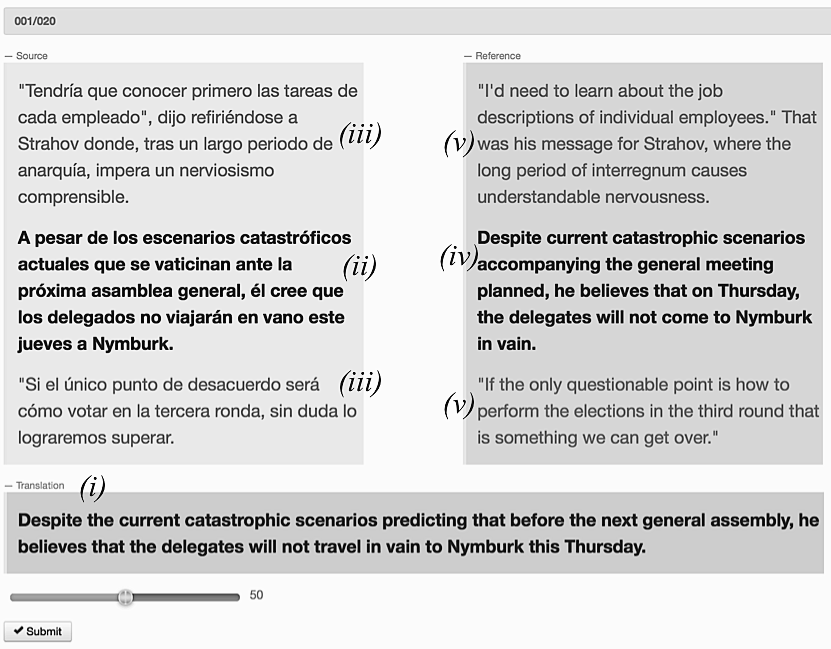
\includegraphics[scale=0.80]{data/EyeAppraiseLayout_srctgt.png}
\caption{Our modified evaluation layout showing: the translation \Ni; the source \Nii, \Niii; the reference \Niv, \Nv; and the scoring \emph{slider}.}
\label{fig:EyeAppraiseLayout}
\vspace{-5pt}
\end{figure*}

 To contrast the effect that different sources of information have on the evaluation procedure, we explored three different evaluation \gamets:
 %\vspace{5pt}

\begin{itemize}
  \item {\bf{Scenario 1}} (\src) shows participants the translated sentence (in English) along with the source text of the translation (in Spanish), including the context of the source sentence (one sentence before and one sentence after the translated sentence). 
  \item {\bf{Scenario 2}} (\srctgt) shows participants the translated sentence (in English), along with the source text of the translation (in Spanish), and a reference translation done by a human (also in English), plus context for both source and reference.  
  \item {\bf{Scenario 3}} (\tgt) shows the translated sentence (in English) only with a reference translation including its context (in English). 
\end{itemize} 
%\vspace{5pt}
%\sout{The source and the reference translation include the context of the sentence, i.e. 1 sentence before and 1 sentence after the sentence.} \stephan{redendant to scenario 1.}\\
%Explain the different layouts that were explored in our experimental design

 %was presented as a number of stars (from 0 to 5). The more stars the closer his score 
 %to the original judgment of the task sentence (See Figure ~\ref{fig:EyeAppraiseLayout}.

\subsection{Feedback}
To keep participants engaged, they were given feedback according to a previously computed quality score for each translation.  This score was calculated using a linear interpolation of the \emph{expected wins} score obtained from the ranking evaluations (normalized to the range [0, 100]) and \discoparty~\cite{discoMT:WMT2014}, a high-performing automatic MT metric based on discourse \cite{discoMT:acl2014}, which won the WMT 2014 metrics task. This was done because expected wins only provide relative scores (i.e. which of two translations is ranked better given the same source sentence), while the participants were evaluating \emph{absolute} scores.
To keep things simple, we provided feedback based on the difference between the evaluator's score and the computed quality scores. Participants were given a five scale feedback depending on the magnitude of these differences ($5$: [0--10], $4$: [11--20], $3$: [21--30], $2$: [31--40], $1$: [$>$40]). In Section~\ref{ss:disc_feedback} we analyze the impact of feedback on the evaluator behavior. %The user was given a feedback about his scoring in reference.


\subsection{Participants}

%The actual experiment was preceded by multiple rounds of pilot experiments involving 4-5 users, including the authors of this article. This step was necessary in order to fine tune the eye-tracker and exclude any external influences such as light embedding the correct recording of the eyes or noise, distracting the participants.

In our experiment we had 20 participants 27 to 45 years old. Seven of the participants were female, and 13 were male. Seventeen of our participants were computer scientists; ten had experience with manually translating documents; and four had experience with machine translation evaluation.  

%Information regarding the use of glasses/lenses (and whether they are anti-reflective) during the experiment was collected. This information was necessary to rule out any interference with the eye-tracker. due to the use of glasses or lenses. 
%Out of the 20 users, 6 wore glasses (5 were anti-reflective), and 2 users wore lenses.% Only in the case of one participant, there was interference with the eye-tracker, which could not correctly track his/her eye movements, so the participant was not taken into account.

All the recruited participants were proficient in English. However, half of the participants were recruited taking into account their mastery of the Spanish Language. For the analysis, participants were divided into two groups of ten people each: 

\begin{itemize}
  \item {\bf{Bilingual}} participants did speak the source language (Spanish) at a native or advance level of comprehension.

  \item {\bf{Monolingual}} participants did not speak the source language. Note that this group included some speakers of other Romance languages. However, the participants insisted that their understanding of Spanish was not enough to correctly comprehend the source text. 
\end{itemize}   

%The participants spoke a variety of other languages (besides the target language English), including: Arabic, Turkish, German, Danish, Bulgarian, Russian, Slovenian, Croatian, Hindi, Chinese, Basque. 
%The number of languages per person varied between 1 and 9 languages.

%A shortcoming of the experiment design was that since Spanish is a \stephan{quite expanded language ???}, our hypothesis was that the speakers of close Romance languages (such as Italian, French, or Portuguese) could partially understand the source language. For this reason, an extensive information regarding the languages participants mastered, and to what extent, was conducted. The speakers of other Romance languages, however, insisted that their knowledge of another romance language was not enough to correctly comprehend the source text in Spanish, so we ruled out this hypothesis.
%\if 0
%Out of the 10 monolingual users, 6 spoke other Romance languages, namely: 

%\begin{itemize}
%  \item 1 user spoke beginner Italian
%  \item 1 user spoke native Italian
%  \item 1 user spoke native Italian and beginner French
%  \item 2 users spoke beginner French
%  \item 1 user spoke native Portuguese
%\end{itemize} 
%\fi

\subsection{Experimental Design}
We planned our experiment to collect $1200$ evaluations, $60$ from each of the $20$ participants.  To do so, we designed an experimental matrix in which we considered the following variables: \Ni evaluator type: \mono, \bil; \Nii length of reference: \lshort, \lmid, \llong; \Niii \gamet: \src, \srctgt, \tgt; and \Niv type of translation: \qmin, \qmax.

In our experimental matrix, each participant evaluated $60$ translations evenly divided into: $20$ translations in each of the \gamet; $20$ translations from each length type; $30$ translations of each quality type. On the other hand, each translation was evaluated by four different participants, two \bil and two \mono.
To avoid any bias, we made sure that each evaluator 
%evaluated the same translation only once (or any other translation coming form the same source sentence). 
saw each source sentence only once.

%Third, we wanted to ensure that each translation is evaluated multiple times by different users.
%Explain the design matrix used. What is the total number of evaluations collected in this round? 1200, 60 per user.


\subsection{\Eye Setup}
%To conduct our experiments, we augmented Appraise ~\cite{federmann2012appraise} -an open-source toolkit ~\footnote{Available at:github.com/cfedermann/Appraise} for translation evaluation. Appraise is based on the Django web framework that uses Twitter's Bootstrap as a model for the interface design. Appraise has four different types of annotation tasks available: \Ni  Ranking (i.e. to say whether translation $A$ is better than translation $B$); \Nii Error Classification, where user classify errors in the translation output as ``minor'' or ``severe'' following \cite{vilar2006error}; \Niii Quality Estimation, where a user determines if the MT output is ``Acceptable'', ``Can easily be fixed'', or neither; and \Niv Post-Editing, where the user chooses a translation which would be the \emph{easiest} to post-edit as described in \cite{avramidis2012}.\\ 

%In our experiments 
%For our experiments, we augmented Appraise to record information from eye tracker. The new Appraise %provided in the project github repository https://github.com/guzmanhe/Appraise/
%includes the capability to interface with eye tracker and record eye information along with the user judgments. 


We used the EyeTribe eye-tracker~\footnote{http://dev.theeyetribe.com/api/} to collect \emph{gaze} information from the participants. The information was sent in messages to a modified version of Appraise\footnote{Available at: https://github.com/Qatar-Computing-Research-Institute/iAppraise} at a rate of 60Hz (a packet in every 16ms). 
%information and communicate the data to the \eye server which serve to broadcast the data/messages read by device to Appraise.  %Communicating with the tracker server is achieved using a connection via a TCP socket that listen to the designated server port (Eyetribe default port 6555). The Tracker API protocol consists of exchanging JSON (JavaScript Object Notation) formatted messages over TCP sockets\ahmed{Figure sample packet}. 
%

Each message contained the gaze position in the screen of both eyes, a flag indicating if the point represented a \emph{fixation}, a time stamp, and other device-related information. 
%a state indicating the status of the tracker. EyeTribe user guide~\footnote{http://dev.theeyetribe.com/api/} details further the structure and the attributes of the messages that can be exchanged with the server. %Figure \ref{fig:EyetribeAPImap}. details the architecture of Appraise. The Eyetribe device was set to operate at a frequency of 60Hz (a reading in every 16ms) which makes it not suitable to track \stephan{high accuracy? Is this the accurate term?} saccades. 
%The screen was configured in a \paco{Ahmed can you add resolution here}, resolution.
%
To ensure optimal readings, participants were asked to calibrate the \eye device before starting the experiments, and a warning message was displayed whenever the eye-tracker lost track of the participant's gaze.
%\begin{figure}[ht]
%\centering
%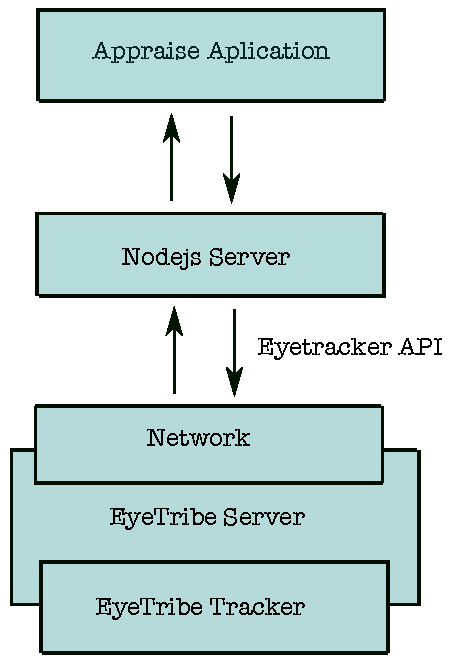
\includegraphics[scale=0.6]{data/EyetrackingAPI.pdf}
%\caption{Eyetribe communication map}
%\label{fig:EyetribeAPImap}
%\end{figure}


%What was the device used for \eye? Can we give more specs (paragraphs only). \paco{@Ahmed}


\subsection{Instructions and Exit Survey}


%
%tuning the eye-tracker required sitting at a certain distance from the computer screen, and looking with both eyes towards the eye-tracking software until the software would recognise both eyes of the participant. 
%Next, the participant had to follow with his/her eyes a moving red circle, in order to train the software to recognise the movement of his eyes. As a third step, the eye-tracking software would show its performance by colouring in red the spots on the screen on which the participant would look at. The objective was to reach 5 stars of calibration, and the software would allow re-calibration if the sufficient quality was not reached (see Figure ?). 

%The latter %The tutorial introducing the experiment 
%would present to the participant the three scenarios and instructions on how to navigate through the screen. %(see Figure? ). 
%
%
Participants were asked to move as little as possible to not interrupt the readings of the eye-tracker, 
%
%
%explicitly asked to not move away from the screen while performing the experiment, as the eye-tracker could lose their eyes. 
%They were also asked 
%
%
and to not interrupt their work while working through the translations belonging to one \gamet, as the time for executing all sentences in one scenario was measured. 
Before conducting the evaluation, participants were shown two tutorials, one showing how to calibrate the eye-tracker and one showing how to conduct the experiment. 

After the tutorials they were asked to perform a warm-up exercise consisting of %2 
two sentences per \gamet.  
%\ahmed{Chop-off all the intro, too much details, no space.}
Then, the participants proceeded to evaluate the $20$ translations in each of the \gamets in the following order \src, \srctgt and \tgt \footnote{In hindsight, randomizing the order in which the \gamets were performed would have allowed to answer an additional set of questions.}.

%What were the considered variables?
%\paco{@Irina}
%\subsubsection{Exit survey}
After the experiment, the participants were asked to fill in an on-line exit survey, which collected their impressions about the experiment and their physiological status during the experiment.

%\begin{itemize}
%  \item Their cognitive state during the experiment (normal, tired, sleepy, sleep-deprived, sick/dizzy);
%  \item The interface;
%  \item The difficulty of evaluating the translation;
%  \item The environment;
%  \item Other.
%\end{itemize}

%A screenshot of the survey form is shown in Figure?. 
From the survey we learned about the physiological state of the participants: $55\%$ of them were in a normal state, $15\%$ were slightly tired or sleepy, $25\%$ were tired, and $10\%$ were sleep-deprived or sick. Yet, all these reports were evenly distributed among \bils and  \monos.
%11 participants were in ``normal'' state, 2 were ``normal, sleepy'', 1 was ``normal, tired'', 5 were ``tired'', out of which 2 were ``tired, sleepy''. 1 was ``sleep-deprived'' and 1 was ``sick/dizzy''. 
%Regarding the interface, participants were mostly content with the experiment {\bf{interface}}, defining it ``clear'', ``simple'', ``easy to use'', and ``very intuitive''. 
%However, $15\%$ of the participants complained of being distracted by a warning message that appeared when they moved away from the eye-tracker,
%the fact some texts where very long %so they had to scroll up and down, 
%or the fact that they had to stay focused on the same screen for too long without moving their eyes.% 3-4 participants also complained of the fact that there were people discussing around them (the experiment was done in an university environment). 

%The perceived \emph{difficulty} of the evaluation task ranged widely among participants (from very easy to hard).

 There were only few complaints about the setup, and they were related to: \Ni the lack of precise instructions of what constitutes a \emph{good} translation, \Nii the large range of the evaluation score (0-100), \Niii the difficulty to understand the context of the translations, and \Niv the cognitive overhead needed to evaluate \llong translations, especially in the \srctgt \gamet. As expected, some of the \mono participants noted that in the \src \gamet they mostly evaluated the readability of the translation, as they had no knowledge of the source language.
\vspace{5pt}

